\documentclass[display,t]{beamer}

\usetheme{Szeged}
\usefonttheme[onlylarge]{structurebold}
\setbeamerfont*{frametitle}{size=\normalsize,series=\bfseries}
\setbeamertemplate{navigation symbols}{}

\usepackage[hungarian]{babel}
\usepackage[utf8]{inputenc}
\usepackage{times}
\usepackage[T1]{fontenc}
\usepackage{listings}
\usepackage{graphicx}
\usepackage{tikz}

\usetikzlibrary{positioning,shapes,shadows,arrows}

\title{Git init}
\subtitle{Bevezetés a Git használatába}
\author{Kiglics Bence}

\begin{document}


\tikzstyle{commit} = [rectangle, draw = black, fill = white, rounded corners,
                      inner sep = 4pt, outer sep = 1pt, text centered,
                      text width = 0.8cm, font=\small]
\tikzstyle{helper node} = [text width = 0.8cm, inner sep = 4pt, outer sep = 1pt]
\tikzstyle{line} = [->, thick, > = stealth]

\tikzstyle{big commit} = [rectangle, draw = black, fill = white, rounded corners,
                          inner sep = 4pt, outer sep = 1pt, text centered,
                          text width=1.5cm, font=\small]
\tikzstyle{big pointer}     = [big commit, fill = lightgray]
\tikzstyle{big head}        = [big commit, fill = darkgray, text = white]
\tikzstyle{big helper node} = [text width = 1.5cm, inner sep = 4pt, outer sep = 1pt]


\frame{\titlepage}


\begin{frame}{Tartalomjegyzék}
    \tableofcontents
\end{frame}



\section{Bevezetés}
\subsection{A verziókövető rendszerek rövid története}
\subsubsection{Korai verziókövetők}


\begin{frame}{Korai verziókövetők}
    \pause
    \begin{block}{SCCS (Source Code Control System)}
        \begin{itemize}
            \pause \item UNIX fejlesztés
            \pause \item Első tapasztalatok
        \end{itemize}
    \end{block}
    \pause
    \begin{block}{RCS (Revision Control System)}
        \begin{itemize}
            \pause \item Csak egyedi fájlokon dolgozik
            \pause \item Diff/patch
            \pause \item Branching
        \end{itemize}
    \end{block}
\end{frame}



\subsubsection{Központosított rendszerek}


\begin{frame}{Központosított rendszerek}
    \pause
    \begin{block}{CVS (Concurrent Versioning System)}
        \begin{itemize}
            \pause \item RCS utódja
            \pause \item Cliens/szerver
        \end{itemize}
    \end{block}
    \pause
    \begin{block}{SVN (Subversion)}
        \begin{itemize}
            \pause \item CVS lecserélésére
            \pause \item HTTP támogatása
        \end{itemize}
    \end{block}
\end{frame}



\subsubsection{Elosztott rendszerek}


\begin{frame}{Elosztott rendszerek}
    \pause
    \begin{block}{BZR (Bazaar)}
        \begin{itemize}
            \pause \item A Canonical Inc. fejlesztése
            \pause \item Launchpad
        \end{itemize}
    \end{block}
    \pause
    \begin{block}{HG (Mercurial)}
        \begin{itemize}
            \pause \item Linux kernel
            \pause \item Binary diff
        \end{itemize}
    \end{block}
\end{frame}



\begin{frame}{Elosztott rendszerek}
    \pause
    \begin{block}{Git}
        \begin{itemize}
            \pause \item Linus Torvalds
            \pause \item A BitKeeper fizetőssé vált
            \pause \item Diff helyett teljes fájlok tárolása
            \pause \item Kis projektekre és hatalmas kódbázisok követésére egyaránt alkalmas
        \end{itemize}
    \end{block}
\end{frame}



\subsection{A verziókövetés alapjai}
\subsubsection{Egy repository működése}


\subsubsection{Egy repository működése}

\begin{frame}{Egy repository működése}
    \pause
    
    \begin{center}
        \begin{tikzpicture}[->, node distance=0.4cm]
            \node (C0) [commit] {C0};
            \pause
            
            \node (C1) [commit, right=of C0] {C1};
            \draw (C0) -> (C1) [line];
            \pause
            
            \node (C2) [commit, right=of C1] {C2};
            \draw (C1) -> (C2) [line];
            \pause
            
            \node (C1to3) [helper node, below=of C1] {};
            \node (C3) [commit, right=of C1to3] {C3};
            \draw (C1) -> (C3) [line];
            \pause
            
            \node (C4) [commit, right=of C2] {C4};
            \draw (C2) -> (C4) [line];
            \pause
            
            \node (C5) [commit, right=of C3] {C5};
            \draw (C3) -> (C5) [line];
            \pause
            
            \node (C6) [commit, right=of C4] {C6};
            \draw (C4) -> (C6) [line];
            \draw (C5) -> (C6) [line];
        \end{tikzpicture}
    \end{center}
\end{frame}



\begin{frame}{Delták}
    \begin{center}
        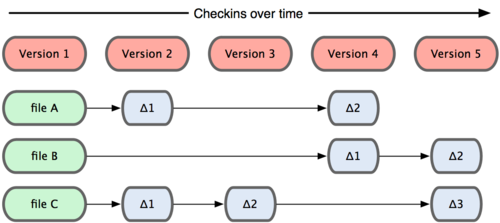
\includegraphics{frames/diagrams/deltas.png}
    \end{center}
\end{frame}



\section{Verziókezelés Git segítségével}
\subsection{A Git felépítése}


\begin{frame}{Git commitok és branchek}
    \begin{center}
        \begin{tikzpicture}[->, node distance=0.5cm]
            \node (C0) [big commit] {0000000};
            
            \node (C1) [big commit, right=of C0] {e95e10e};
            \draw (C1) -- (C0) [line];
            
            \node (C2) [big commit, right=of C1] {eea4ec7};
            \draw (C2) -- (C1) [line];
            
            \node (C3) [big commit, right=of C2] {421409f};
            \draw (C3) -- (C2) [line];
            
            \node (C1to4) [big helper node, below=of C1] {};
            \node (C4) [big commit, right=of C1to4] {8eddc0a};
            \draw (C4) -| (C1) [line];
            \pause
            
            \node (master) [big pointer, above=of C3] {master};
            \draw (master) -- (C3) [line];
            \pause
            
            \node (branch) [big pointer, below=of C4] {branch};
            \draw (branch) -- (C4) [line];
            \pause
            
            \node (HEAD) [big head, above=of master] {HEAD};
            \draw (HEAD) -- (master) [line];
        \end{tikzpicture}
    \end{center}
\end{frame}



\begin{frame}{Kommitok}
    \begin{center}
        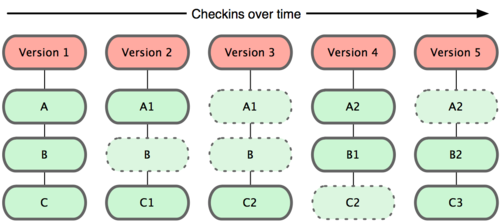
\includegraphics{frames/diagrams/commits.png}
    \end{center}
\end{frame}



\begin{frame}{Blobok}
    \begin{center}
        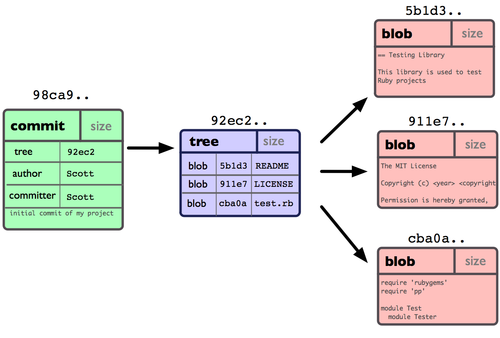
\includegraphics{frames/diagrams/blobs.png}
    \end{center}
\end{frame}



\begin{frame}{Blobok}
    \begin{center}
        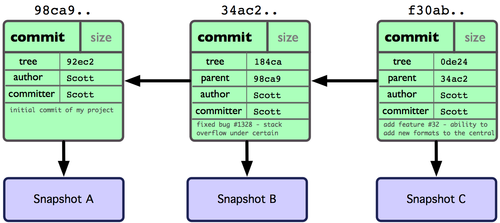
\includegraphics{frames/diagrams/refs.png}
    \end{center}
\end{frame}



\subsection{Git lokális utasítások}


\begin{frame}[fragile]{Git repository inicializálása}
    \pause
    Inicializálás\small
\begin{verbatim}
~/myproject$ git init
Initialized empty Git repository in ~/myproject/.git/
\end{verbatim}
    \normalsize
    
    \pause
    "Bare" repository inicializálás\small
\begin{verbatim}
~/myproject$ git init --bare
\end{verbatim}
    \normalsize
\end{frame}



\begin{frame}{Git fájl állapotok}
    \begin{center}
        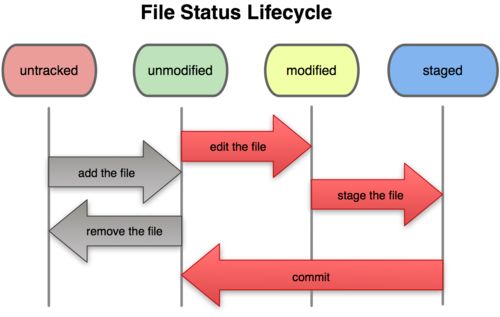
\includegraphics{frames/diagrams/state-lifecycle.png}
    \end{center}
\end{frame}



\begin{frame}[fragile]{Git fájl állapotok}
    \pause
    \begin{center}
        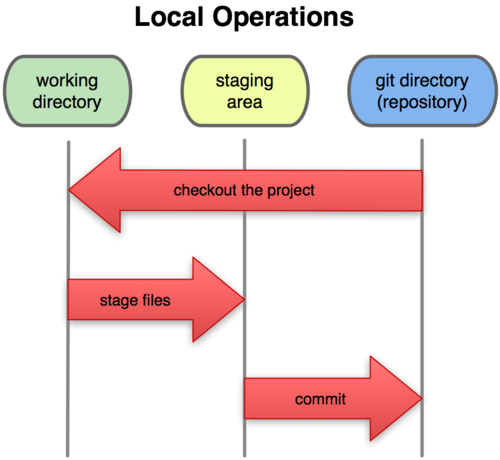
\includegraphics[width=3cm]{frames/diagrams/three-states.png}
    \end{center}
    
    \pause
    Unstaged fájlok staged állapotba helyezése:
\begin{verbatim}
~/myproject$ git add file.txt
\end{verbatim}

    \pause
    Staged fájlok unstaged állapotba helyezése:
\begin{verbatim}
~/myproject$ git rm --cached file.txt
rm 'file.txt'
\end{verbatim}
\end{frame}



\begin{frame}[fragile]{Git állapot vizsgálata}
    Beszédes kimenet
    \tiny
\begin{verbatim}
~/myproject$ git status
# On branch master
# Changes not staged for commit:
#   (use "git add <file>..." to update what will be committed)
#   (use "git checkout -- <file>..." to discard changes in working directory)
#
#	modified:   Makefile
#	modified:   git-presentation.tex
#
no changes added to commit (use "git add" and/or "git commit -a")
\end{verbatim}

    Napló lekérdezése:
\begin{verbatim}
~/myproject$ git log [--oneline] [--graph]
\end{verbatim}

    Változások lekérdezése:
\begin{verbatim}
~/myproject$ git diff
\end{verbatim}
\end{frame}



\begin{frame}[fragile]{Git commit}
    \pause
    Csak staged fájlok commitja:
\small\begin{verbatim}
~/myproject$ git commit -m "message"
[master 08e617f] message
 1 file changed, 135 insertions(+), 13 deletions(-)
\end{verbatim}\normalsize
    \pause
    
    Repóban szereplő módosult fájlok commitja:
\small\begin{verbatim}
~/myproject$ git commit -a -m "message"
\end{verbatim}\normalsize
    \pause

    Fájlok revertálása:
\small\begin{verbatim}
~/myproject$ git checkout HEAD file.txt
\end{verbatim}\normalsize
\end{frame}



\begin{frame}[fragile]{Git branchek}
    \pause
    Branch létrehozása:
\small\begin{verbatim}
~/myproject$ git branch new_branch
\end{verbatim}\normalsize

    \pause
    Branchre váltás:
\small\begin{verbatim}
~/myproject$ git checkout new_branch
\end{verbatim}\normalsize

    \pause
    Egy utasításban:
\small\begin{verbatim}
~/myproject$ git checkout -b new_branch
\end{verbatim}\normalsize
\end{frame}



\begin{frame}[fragile]{Git branchek}
    \pause
    Branch mergelése:
\small\begin{verbatim}
~/myproject$ git merge mergable_branch
\end{verbatim}\normalsize

    \pause
    Javasolt eszközök:
    \begin{itemize}
        \item meld (*nix)
        \item kdiff3 (*nix, Windows)
        \item opendiff (Mac)
    \end{itemize}
\end{frame}



\subsection{Verziókezelés a felhőben}

\begin{frame}[fragile]{Távoli utasítások}
    \pause
    Repó klónozása:
\small\begin{verbatim}
~/myproject$ git clone <repository>
\end{verbatim}\normalsize

    \pause
    Távoli változások begyűjtése:
\small\begin{verbatim}
~/myproject$ git fetch [reponame]
\end{verbatim}\normalsize

    \pause
    Begyűjtés és merge egy lépésben:
\small\begin{verbatim}
~/myproject$ git pull [reponame]
\end{verbatim}\normalsize

    \pause
    Lokális commitok szinkronizálása a szerverre:
\small\begin{verbatim}
~/myproject$ git push [reponame]
\end{verbatim}\normalsize
\end{frame}



\begin{frame}[fragile]{Távoli utasítások}
    \pause
    Új távoli repó hozzáadása és törlése:
\small\begin{verbatim}
~/myproject$ git remote add <reponame> <location>
~/myproject$ git remote rm <reponame>
\end{verbatim}\normalsize
\end{frame}



\begin{frame}[fragile]{Stash}
    \pause
    "Dirty" állapot stashbe helyezése
\small\begin{verbatim}
~/myproject$ git stash
\end{verbatim}\normalsize

    \pause
    Stashben lévő állapot kiemelése
\small\begin{verbatim}
~/myproject$ git (pop|apply)
\end{verbatim}\normalsize

    \pause
    Stash állapot törlése
\small\begin{verbatim}
~/myproject$ git stash drop <stashid>
\end{verbatim}\normalsize

    \pause
    Stashből új branch kiemelése
\small\begin{verbatim}
~/myproject$ git stash branch <branch_név>
\end{verbatim}\normalsize
\end{frame}



\section{További információ}
\subsection{Git eszközök}


\begin{frame}{Git eszközök}
    \begin{itemize}
        \item gitk (*nix, Mac)
        \item git-cola
        \item GitHub for Windows/Mac
        \item TortoiseGit (Windows)
    \end{itemize}
\end{frame}



\subsection{Linkek, elérhetőségek}


\begin{frame}{Linkek, elérhetőségek}
    \begin{itemize}
        \item http://git-scm.com/book
        \item http://teach.github.com/
        \item http://mac.github.com/
        \item http://windows.github.com/
        \item http://code.google.com/p/tortoisegit/
    \end{itemize}
\end{frame}



\begin{frame}
    \begin{center}
        
\includegraphics[width=6cm]{approved_by_csibi.png}
    \end{center}
\end{frame}



\end{document}

